% Parte 5: DTI004, recuperacao completa, Metodo 1 x Camps.
% problems/camps_dti004/outputs/set1/SUMMARY.md e truth5ti_s*_{m1,camps}.json
% (2026-10-13); tabela e figura: scripts/deck_figs.py.

\section{DTI004: recuperação completa}

\begin{frame}{DTI004: Método 1 $\times$ Camps}
  \small
  \begin{itemize}\setlength{\itemsep}{0.3em}
    \item Seis verdades, cada uma com 5 root nodes em $t = 0$ entre os 601 candidatos de Camps; velocidades a $\pm 1\%$ da verdade nos dois métodos.
    \item \textbf{Camps}: SMC-ABC, 512 partículas; mapas por Dijkstra, discrepância de ECG por DTW; 16 núcleos de CPU.
    \item \textbf{Método 1}: 100 inicializações $\times$ 1000 iterações; mapas por FIM, ECG por lead field; uma GPU.
    \item Cada método contra a sua própria verdade (Dijkstra $\times$ FIM). O erro de ECG é a nossa métrica, não a que Camps otimiza.
  \end{itemize}
\end{frame}

\begin{frame}{Resultados por verdade}
  \centering
  \tiny
  \setlength{\tabcolsep}{3.6pt}
  \renewcommand{\arraystretch}{0.92}
  \begin{tabular}{@{}llcccccccccc@{}}
    \toprule
    verdade & método & soluções & \shortstack{tempo\\(min)} & corr & \shortstack{LAT MAE\\(ms)} & ECG & \shortstack{root\\nodes} & \shortstack{verdade $\to$\\recup.\ (cm)} & \shortstack{recup.\ $\to$\\verdade (cm)} & \shortstack{$\geq 2$ roots\\a $\leq 1$ cm}\\
    \midrule
\inputrows{sections/tab_dti004.tex}
    \bottomrule
  \end{tabular}\par
  \medskip
  {\tiny Medianas sobre as soluções (partículas ou inicializações). verdade $\to$ recup.: média, sobre os 5 root nodes verdadeiros, da distância geodésica ao recuperado mais próximo;
  recup.\ $\to$ verdade: o inverso. Root nodes: candidatos ativos (Camps); fontes com profundidade $\geq 1$ ms (Método 1).
  Última coluna: fração das soluções com ao menos 2 root nodes verdadeiros a até 1 cm.}
\end{frame}

\begin{frame}{Todas as soluções das seis verdades}
  \centering
  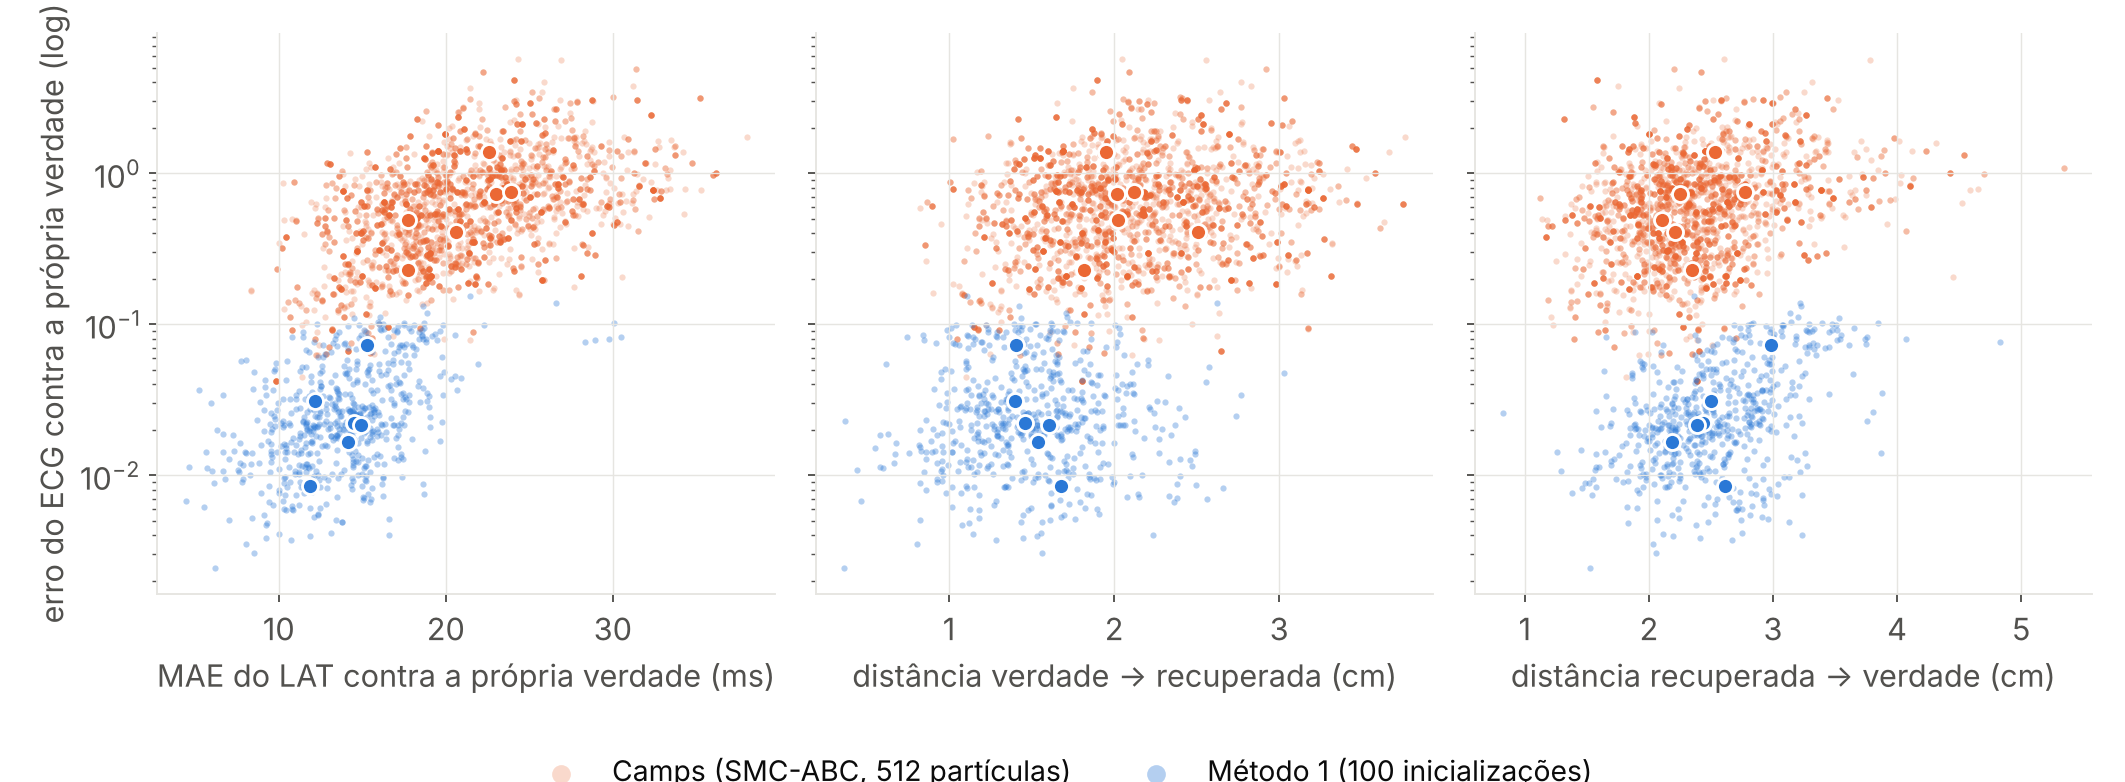
\includegraphics[width=\linewidth]{dti004_membros.png}\par
  \smallskip
  {\scriptsize Pontos: cada solução; círculos grandes: a mediana de cada verdade.}
\end{frame}
